\appendix


\chapter{Anexos del Desarrollo}\label{ac:desarrollo}
\newpage
\section{Enlaces de Interés}
Los enlaces se agregaron el día 13/08/2021.
\begin{enumerate}
    \item El enlace donde se desarrolló el front end del sistema es : \url{https://github.com/agustinbritez/Sistema_Validacion.git}.
    \item Enlace de Smart Contract publicado en Ropsten: \url{https://ropsten.etherscan.io/address/0x7006882779C21D8246C82989F813237f78A781b1}
    \item Enlace de Remix : \url{https://remix.ethereum.org/}
    \item Enlaces de páginas grifos (obtener ETH en Ropsten) : \url{https://faucet.metamask.io/} o \url{https://faucet.ropsten.be}.
\end{enumerate}

\section{Métodos de relevamientos}

Para relevar información acerca de la facultad, se realizó una entrevista formal mediante comunicación remota  con el encargado de la Secretaría de Extensión, también comunicación informal mediante
chats, y observaciones, se utilizó documentos referenciados en la bibliografía como el estatuto de la \gls{unam}.

% \section{Imágenes del proceso de prueba} \label{as:imagenes_pruebas}
% 
Los modelos de los certificados fueron extradidos del sitio web vecteezy.com \href{https://static.vecteezy.com/ti/vetor-gratis/p3/2252202-blue-and-gold-certificate-of-achievement-template-set-background-with-gold-badge-and-border-award-diploma-design-blank-vector-illustration-eps10-gr%C3%A1tis-vetor.jpg}{Imagen del modelo del certificado}
   \begin{figure}[H]
    \centering
    {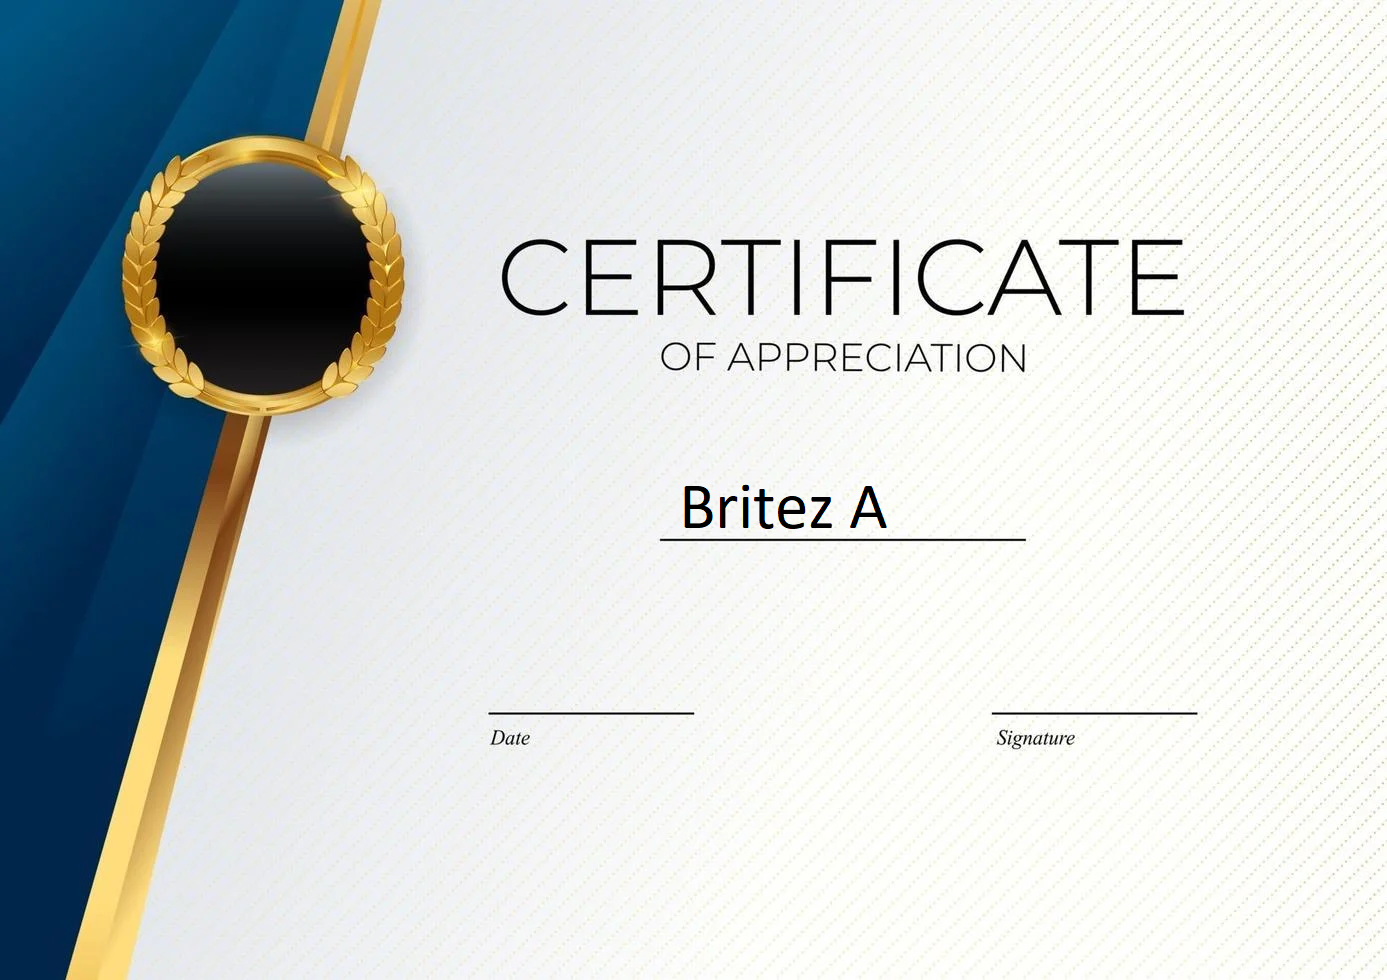
\includegraphics[scale=0.4]{certificado_1.png}}
    \caption{certificado\_1 con hash 8c512569046860bcd 303a11b9b87da4686c63 c5dcac38619084fbe8a2fa31749 , captura de pantalla del Autor}
    \label{img:certificado_1}
  \end{figure}

   \begin{figure}[H]
    \centering
    {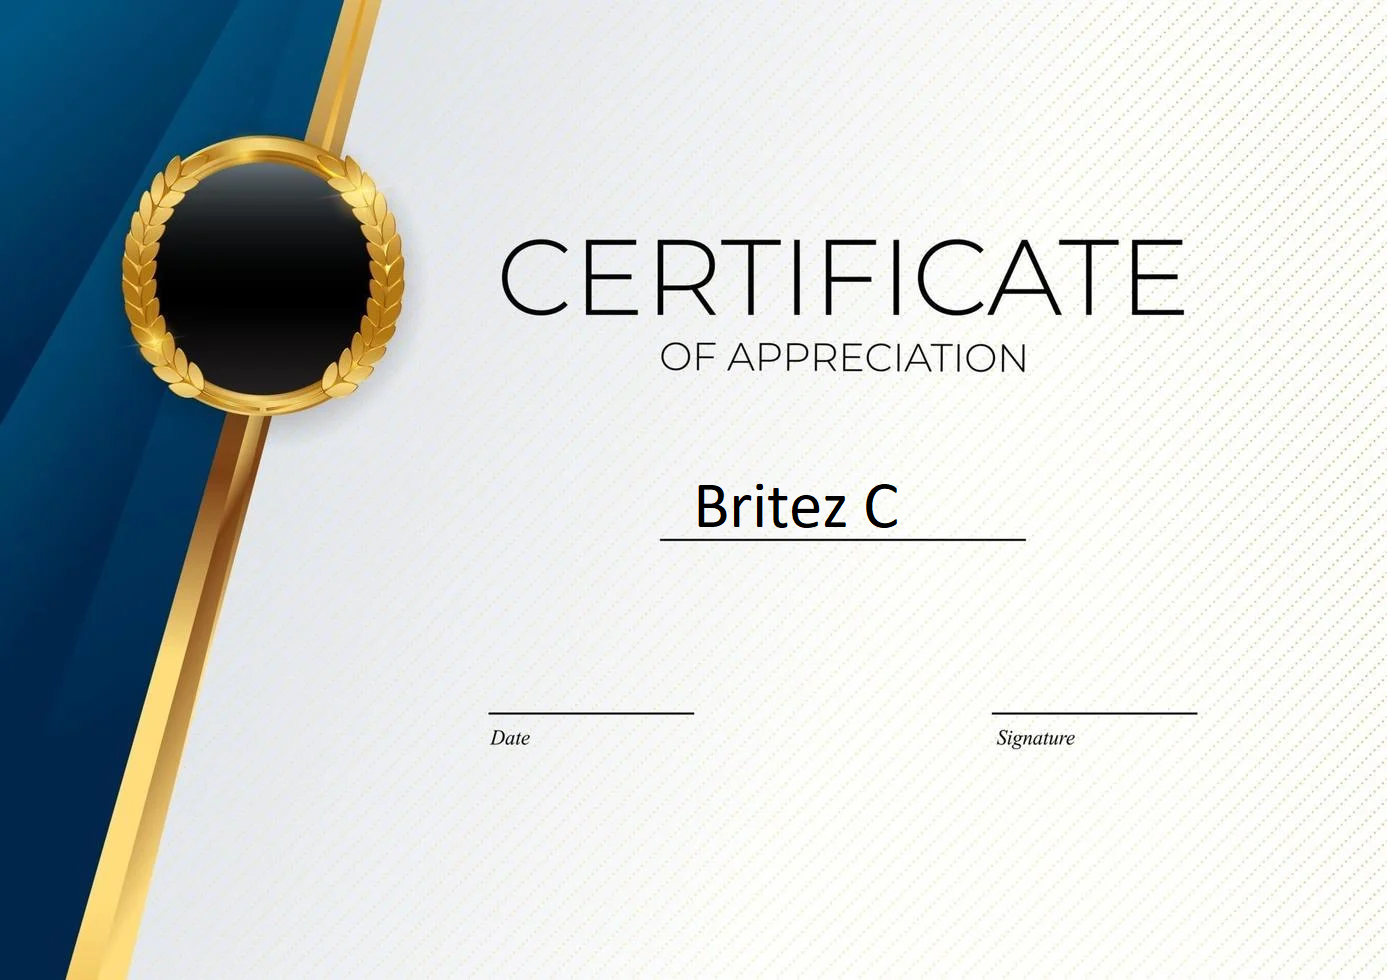
\includegraphics[scale=0.4]{certificado_2.png}}
    \caption{certificado\_2 con hash 06196dfac36f 3b97bab6b4f75ebab20e0e129d627 f1d4202cbb337e446fb6380, captura de pantalla del Autor}
    \label{img:certificado_2}
  \end{figure}

   \begin{figure}[H]
    \centering
    {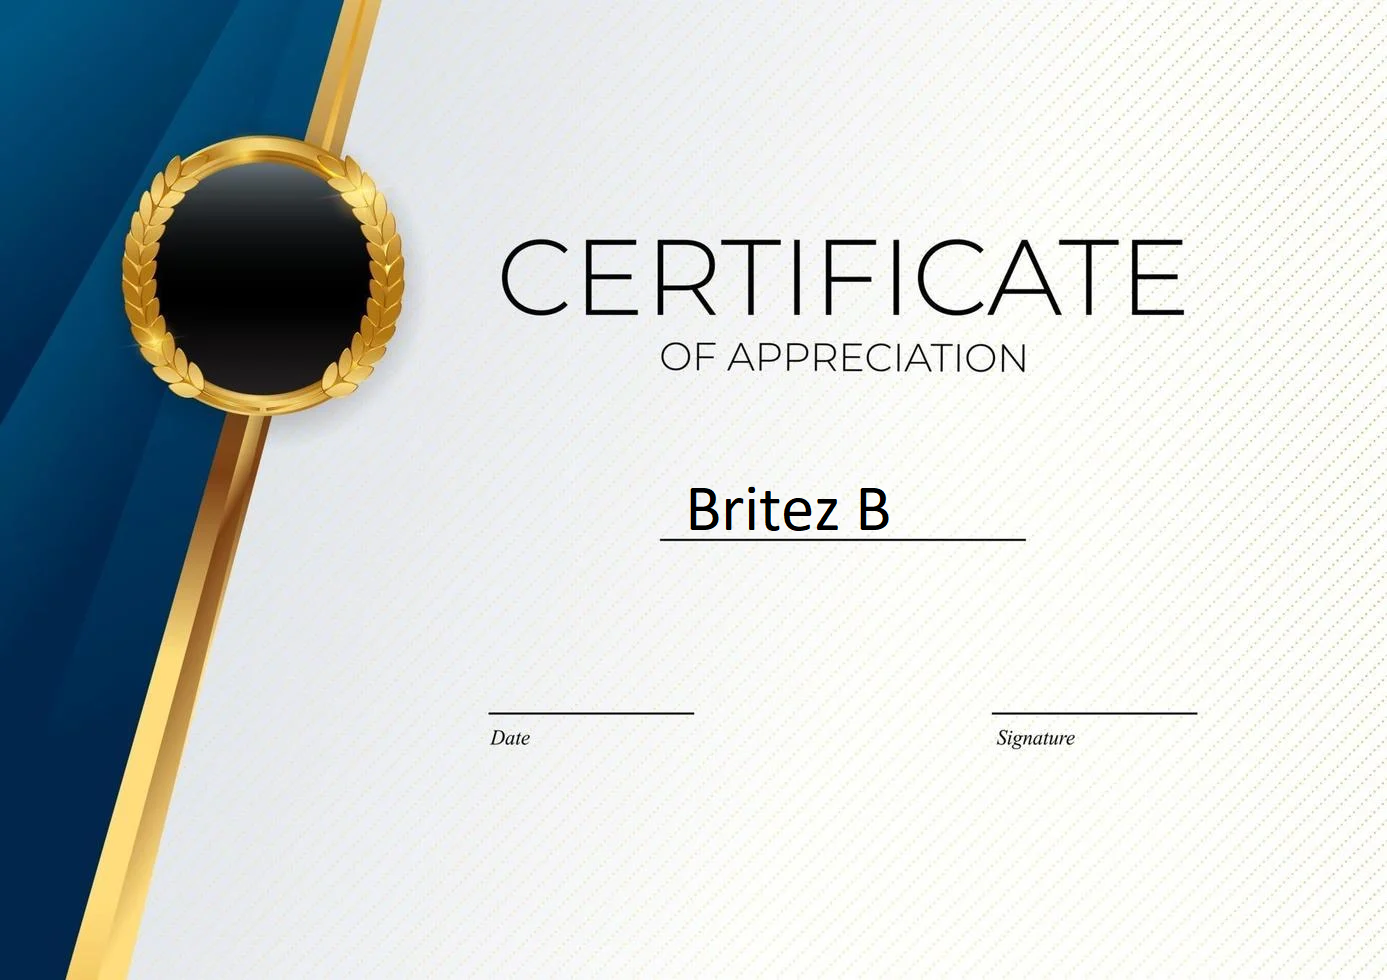
\includegraphics[scale=0.4]{certificado_3.png}}
    \caption{certificado\_3 con hash 20f1185242b6dc594f 5f04f5777cc318b070d244b9b4 b7b2aa0e9383a412ce7b, captura de pantalla del Autor}
    \label{img:certificado_3}
  \end{figure}


% \section{Elementos de Prueba} \label{as:elementos_prueba}
% 
Las imágenes denominadas imagen1.png, imagen2.png se insertaron pequeños cambios que podrían pasar desapercibido.

\begin{figure}[H]
    \centering
    {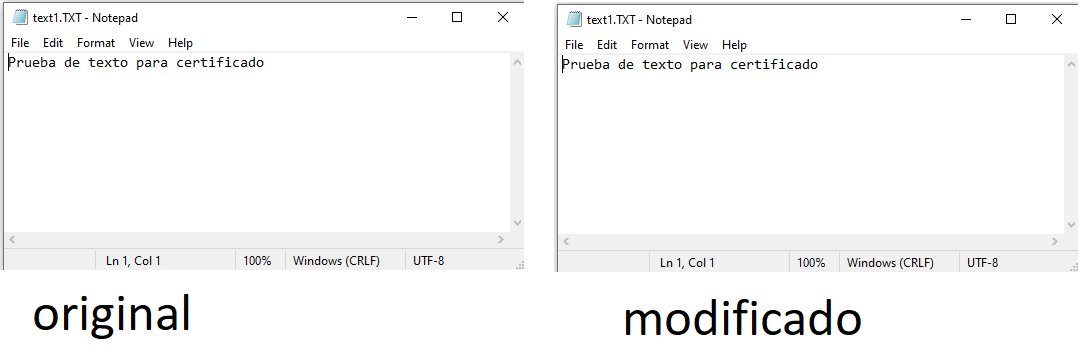
\includegraphics[scale=0.6]{prueba_imagen_comparacion_text1.png}}
    \caption{El cambio está dentro de la primer  “ d ” se agrego un punto}
    \label{img:comparacion_tex1}
\end{figure}
\begin{figure}[H]
    \centering
    {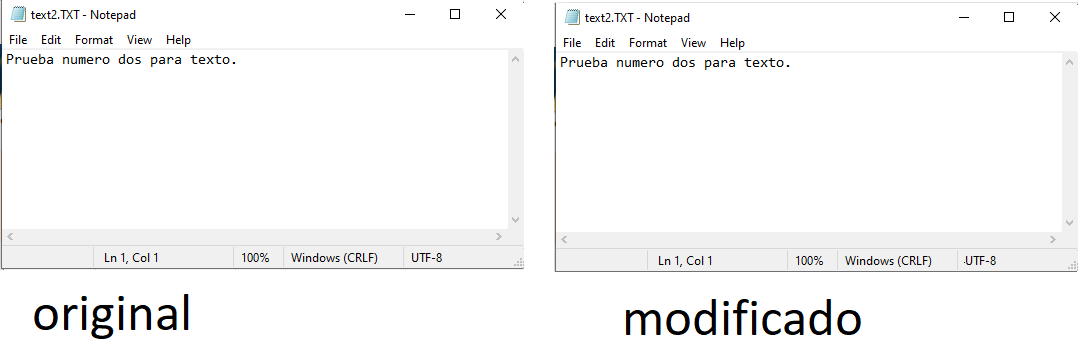
\includegraphics[scale=0.6]{prueba_imagen_comparacion_text2.png}}
    \caption{El cambio es en la parte inferior derecha donde se encuentra escrito “UTF-8”}
    \label{img:comparacion_tex2}
\end{figure}
En cambio en las otras imágenes es más evidente la modificaciones voluntarias.
\begin{figure}[H]
    \centering
    {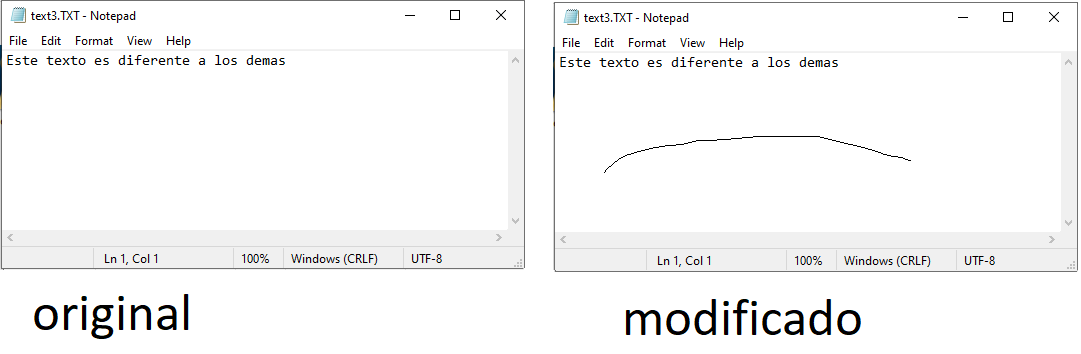
\includegraphics[scale=0.6]{prueba_imagen_comparacion_text3.png}}
    \caption{Imagen text3.png comparación }
    \label{img:comparacion_tex3}
\end{figure}
\begin{figure}[H]
    \centering
    {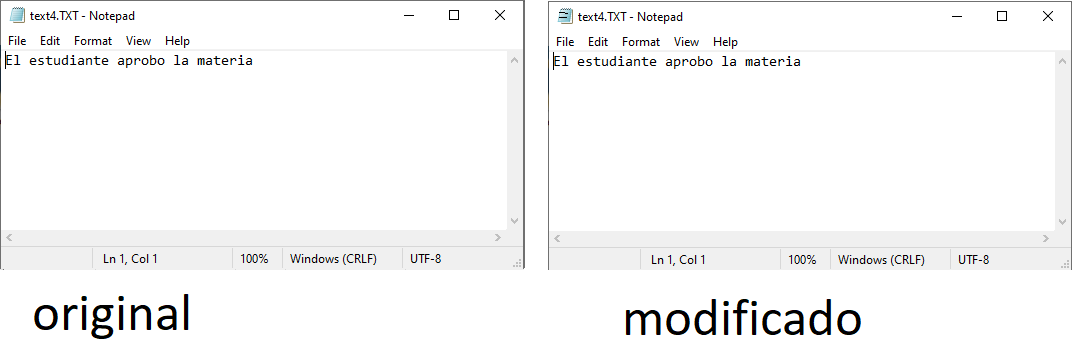
\includegraphics[scale=0.6]{prueba_imagen_comparacion_text4.png}}
    \caption{Imagen text4.png comparación }
    \label{img:comparacion_tex4}
\end{figure}
\begin{figure}[H]
    \centering
    {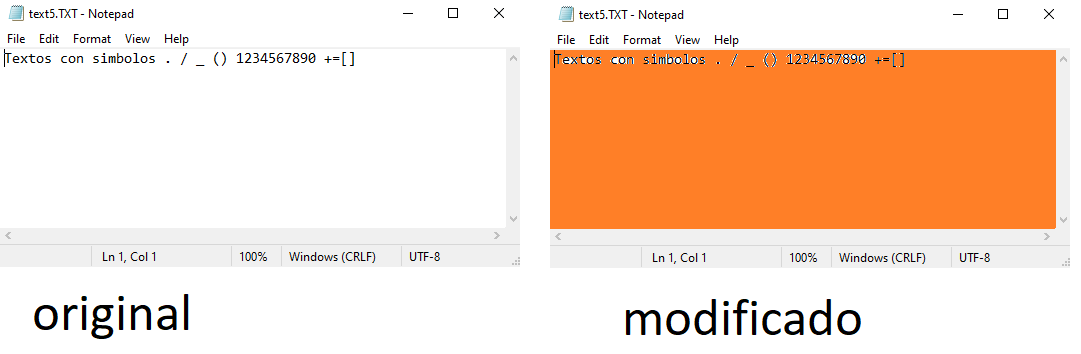
\includegraphics[scale=0.6]{prueba_imagen_comparacion_text5.png}}
    \caption{Imagen text5.png comparación }
    \label{img:comparacion_tex5}
\end{figure}

\section{Comunicaciones Personales y Observaciones}

Se realizó charlas personales con el encargado de la Secretaría de extensión de la \gls{fce}, se realizó una entrevista, 
y conversaciones por mensaje de textos los dias 02,03,04 de octubre del 2021.

Las observaciones realizadas en la \gls{fceqyn} y \gls{fce} también sirvieron como aporte para el entendimiento del trabajo realizado por las ambas facultades.  


\subsection{Etrevista a Responsable de la Secretaría de Extensión de la Facultad de Ciencias Económicas}
La entrevista fue realizada el 2 de Octubre del 2020, la información personal del entrevistado se mantiene anónimo. 

\begin{enumerate}
    \item ¿Actualmente que actividades debe realizar la Secretaría de Extensión?.
    
    
    Se encarga de participar en cualquier evento o actividad que sea necesario la interacción con individuos académicos, no académicos, el objetivo 
    principal es conectar, educar y debatir con exterior de la facultad, por ello se dictan cursos, eventos, charlas y no todos ellos son específicamente dedicado a estudiantes universitarios.
    Hay casos de capacitaciones que hemos hecho inclusive a empleados de algunas empresas de la región.
    El objetivo es incrementar los conocimientos del ambiente que rodea la universidad en sí.
    La gestión y logística de todos los materiales necesarios para efectuar una la charla o evento.
    Encargado de la coordinación de los eventos que  certifiquen  cualquier actividad que se requiera, como certificaciones a charlas, congreso.
    Para iniciar un evento por parte de algún docente, no docente, funcionarios o secretarios deben tener la aprobación mediante algún instrumento.



    \item ¿Que significan los instrumentos?
    
    
    Los instrumentos son los registros sobre la aprobación
    de algún evento mediante las disposiciones o resoluciones, estos documentos
    también impulsan la generación de las actividades.

    Pero por otro lado para la aprobación de algún evento se 
    pueda llevar en marcha es necesario que estos estén dentro
    del marco de programa o proyecto. Por lo general cuando hablamos de programas son los planes 
    esperados a largo plazo. Mientras que los proyectos, 
    son parte de los programas para el cumplimiento de objetivos en
    plazos más cortos. 
    Entonces para que un evento sea aprobado debe encontrarse dentro de 
    los planes de la universidad. 

    Si la actividad propuesta no está alineado a los planes o programas,
    la única opción es que sea aprobada mediante la disposición del decano. 

    Una vez aprobado el evento, se realiza toda la logística, 
    en caso de que el evento sea muy grande se reservan las 
    aulas más grandes, se establecen fechas para efectuar el evento,
    se calculan los presupuestos.
    Se planea la cantidad de tiempo que durara, etc.

    Los eventos pueden ser congresos, charlas o cualquier actividad que se plante,
    puede haber diferentes charlas en un evento y recibir un certificado por 
    cada una que asistió o simplemente un certificado para todas.



     
    \item ¿Que documentación o tipo de documentos utilizan o manejan? (formato papel o digital).
   
   
    Gestionamos documentos desde la parte del docente, alumnos, y no docentes, ya que la creación de una actividad puede venir desde el grupo de alumnos, como del docente o inclusive personal 
    no académico. Los documentos son por lo general en formato físico o papel, pero también con la situación de la cuarentena se empezó a utilizar el token con pendrive,
    que nos permite enviarnos documentos digitales con las firmas de las autoridades. Los documentos son para la creación de algún evento en particular, para las peticiones de materiales o herramientas, 
    también debemos hacer informes para reservar lugares de los eventos para una fecha específica, por otro lado manejamos la gestión de los certificados de los estudiantes
    que participan en una actividad o también a los disertantes. 
    
    Por último también se presentan presupuestos que conlleva realizar las actividades o los eventos en la facultad se manejan distintos tipos de documentos, pero en nuestra área con frecuencia
    empleamos para la gestión de una actividad.


    
    \item ¿Como se gestionan los eventos o actividades?
    
    Como dije anteriormente un evento puede ser iniciado por parte de un estudiante, docente o personal no docente, pero para ello
    la actividad debe formar parte de un programa de la facultad o estar en disposiciones o resoluciones, 
    no obstante para que el proyecto sea aprobado se necesita que estén alindados a los fines de la facultad, en casos
    que la actividad sea extraordinaria se evalúa por los responsables de la Secretaría de Extensión para rechazarla o aprobarla.

    Cuando la actividad o el evento es aprobado, el personal administrativo inicia con las elevaciones para 
    la gestión del sitio donde se van a realizar los eventos, inicia con los preparativos para seleccionar a los 
    expositores o disertantes, la duración del evento, la publicidad, marketing, con todos los preparativos que son necesarios para el evento.
    Hay casos que son eventos como una juntas cortas, que no necesitan mucha gestión y por otro lado eventos enormes que hay que movilizar muchos sectores.
    


    

    \item ¿La certificación de los eventos o actividades como se realizan?
    
   
    Anteriormente, se realizaban eventos o actividades donde no se entregaban
    certificados, pero como resultado ¿qué sucedió?, disminuyo significativamente
    el número de participantes, entonces se volvió a la entrega de certificados.

    Los certificados pueden ir dirigidos a cualquier individuo, tanto 
    como estudiantes, docentes, no docentes. Porque la actividad 
    se ejecuta para un público en particular o para todo público dependiendo el caso.

    Para que los participantes puedan constatar que han asistido a un evento, se 
    le entregan certificados, que pueden ser de asistencias, por exámenes, o 
    cualquier actividad que se haya planificado para el evento.

    Para la certificación lo que hacemos es tomar los datos de los posibles participantes
    primero creando un formulario de Google  y publicándolo en todas nuestras redes sociales,
    antes este registro se hacía manualmente y nos consumía mucho tiempo. Sin embargo
    con la utilización de esta herramienta nos facilitó mucho la obtención de datos.
    A veces nos piden que hagamos estadísticas si la cantidad de participantes 
    son estudiantes, docentes o no docentes. En otros casos, estadísticas de edades, 
    si trabajan o estudian y con el Google formulario podemos hacerlo de una manera
    más eficiente. 



    \item ¿Cual es el proceso que realizan para emitir los certificados ?
 
   
    Los procesos que realizamos para emitir los certificados son los siguientes:

    Unos días antes del evento se hace el modelado de los certificados, por ejemplo se toma
    un modelo antiguo o se crea uno nuevo donde se deja sin completar los espacios de las firmas y datos de los
    participantes. Después lo que hacemos es pedirle a las autoridades es firmas escaneadas para integrarlas al modelo 
    del certificado, también nos encargamos de la gestión del lugar, conseguir
    los disertantes etc. Pero siguiendo con el proceso como mencione, se hace publicidad del evento
    mediante una página o se usa las redes sociales para anunciar las fechas del evento y un link o un formulario de Google
    para que los estudiantes se puedan registrar, no todos los eventos son de entrada libre, algunos hay que 
    comprar las entradas.
    El día del evento se vuelven a verificar los usuarios que asistieron, para preparar 
    los certificados con los datos de los usuarios que asistieron.  
    Al finalizar el evento se entrega a los participantes el certificado de asistencia y en caso de que sea necesario
    los certificados de exámenes aprobados, estos certificados en algunos casos lo imprimimos y entregamos a 
    los participantes, en otras situaciones hemos entregado de manera digital mediante correo electrónico.
    Para los certificados de examen aprobados, si son pocos participantes se entrega en el mismo evento,
    pero por lo general tarda un poco más de tiempo evaluarlos. 



    \item ¿Que problema puede percibir en cuanto a la validación de los certificados?
    
   
    Sabemos que el tipo de validación mediante  las firmas escaneadas no representan un método muy
    fiable para validar los documentos porque alguien que maneje un poco de informática puede editar los datos.
    Sería necesario tener algún método  para poder validar los certificados de manera sencilla, porque tampoco es conveniente complicar
    aún más el proceso de certificación.

    \item ¿En el caso que algún estudiante quiera revalidar un certificado emitido hace tiempo, como lo hacen?
    
    En esos casos generalmente el estudiante se acerca con el certificado y lo sellamos para dar validez al certificado, pero si el certificado es virtual se busca en
    nuestra base de datos y lo volvemos a enviar a su correo, o si el certificado no lo toman como válido se lo imprime y se lo sella pero eso sucede
    casos particulares.





\end{enumerate}



\newpage
\section{Código Smart Contract} \label{as:codigo_smart_contract}
\begin{verbatim}

    // SPDX-License-Identifier: GPL-3.0
    pragma solidity >0.5.99 <0.8.0;
    pragma experimental ABIEncoderV2;
    
    contract validationSystem {
        /***************Modifier************** */
    
        modifier onlyOwnerOrg() {
            require(
                ownerOrg == msg.sender,
                "Only  Organitation Owner can call this function"
            );
            _;
        }
    
        //**************Struct*************** */
    
        struct Area {
            uint256 id;
            // bool editable;
            address ownerArea;
            string name;
            string description;
            uint256 state_id;
            uint256[] idEvents;
        }
    
        // name= Verificado mean= El documento esta verificado
        struct State {
            uint256 id;
            string name;
            string mean;
        }
        // mapping (uint256=>string) Reason;
        struct Document {
            //hash
            string idHash;
            uint256 state_id;
            uint256 event_id;
            //date of expired timestamp
            uint256 expiration;
            string reasonState;
            //new Version of document
            string newDocument;
        }
    
        struct Event {
            uint256 id;
            string name;
            string description;
            uint256 state_id;
            string startEvent;
            string endEvent;
            //Propietario que puede hacer cambios al evento
            uint256 area_id;
            //storage idhash
            string[] idDocuments;
        }
        //*************************  ************* */
        // only one organitation   for avoid that use a smart 
        contract for  upload many files
        string private organitaton;
    
        address private ownerOrg;
        //all states
        State[] private states;
        //one owner many areas
        mapping(address => uint256[]) public ownerArea;
        //all areas
        Area[] private areas;
        //all events
        Event[] private events;
        // hash => document
        mapping(string => Document) private documents;
    
        /**************** Methods ***************** */
        constructor() {
            ownerOrg = msg.sender;
            uint256[] memory idEvents;
            //La primer area todos las areas borradas hacen 
            referencia a este
            Area memory zero = Area(0, address(this), "null", 
            "null", 1, idEvents);
            areas.push(zero);
    
            State memory _state = State(0, "deleted", "deleted");
            State memory _state2 = State(1, "actived", "actived");
            State memory _state3 = State(2, "expired", "expired");
    
            states.push(_state);
            states.push(_state2);
            states.push(_state3);
            string[] memory str;
            Event memory _event = Event(0, "null", "null", 0, "", "",
             zero.id, str);
            events.push(_event);
        }
    
        /*********************Organitation************************* */
        function setOrganitation(string memory org) public payable 
        onlyOwnerOrg {
            organitaton = org;
        }
    
        function editOwnerOrg(address newOwner) public payable 
        onlyOwnerOrg {
            ownerOrg = newOwner;
        }
    
        /******************State************************ */
    
        function addState(string memory name, string memory mean)
            public
            payable
            onlyOwnerOrg
            returns (uint256)
        {
            uint256 id = states.length;
            State memory newState = State(id, name, mean);
            states.push(newState);
            return id;
        }
    
        function editState(uint256 id,string memory name,string 
        memory mean)
            public
            payable
            onlyOwnerOrg
            returns (
                uint256,
                string memory,
                string memory
            )
        {
            require((states.length > id) && (id > 1));
            (states[id].name = name);
            (states[id].mean = mean);
            return (id, states[id].name, states[id].mean);
        }
    
        /***************Area************************* */
        function addArea(address _ownerArea,string memory _name,
        string memory _description) public payable onlyOwnerOrg {
            uint256 _id = areas.length;
            uint256[] memory _events;
            Area memory _newOwner =
                Area(_id, _ownerArea, _name, _description, 1, 
                _events);
    
            areas.push(_newOwner);
            ownerArea[_ownerArea].push(_id);
        }
    
        function editArea(uint256 _id_area,string memory _name,
        string memory _description,uint256 _id_state) public 
        payable {
            require(
                (ownerOrg == msg.sender) ||
                    (areas[_id_area].ownerArea == msg.sender)
            );
    
            if (bytes(_name).length > 0) {
                areas[_id_area].name = _name;
            }
    
            if (bytes(_description).length > 0) {
                areas[_id_area].description = _description;
            }
            if (_id_state < states.length) {
                areas[_id_area].state_id = _id_state;
            }
        }
    
        function changeOwnerArea(uint256 _id_area, address 
        _newOwner)
            public
            payable
            onlyOwnerOrg
        {
            require((areas.length > _id_area) && (_id_area > 0));
            //get oldest owner
            address _oldOwner = areas[_id_area].ownerArea;
            //changue oldest area_id by 0
            for (uint256 index = 0; index < ownerArea[_oldOwner]
            .length;index++) {
                if (ownerArea[_oldOwner][index] == _id_area) {
                    ownerArea[_oldOwner][index] = 0;
                    break;
                }
            }
    
            ownerArea[_newOwner].push(_id_area);
            areas[_id_area].ownerArea = _newOwner;
        }
    
        /********************Event***************************** */
    
        function addEventFull(uint256 _area_id,string memory name,
        string memory description,string memory _startDate,
        string memory _endDate) public payable returns (uint256 id)
         {
            require(
                (areas[_area_id].ownerArea == msg.sender) ||
                    (ownerOrg == msg.sender)
            );
    
            uint256 _id = events.length;
            string[] memory _document;
    
            Event memory evento =
                Event(
                    _id,
                    name,
                    description,
                    1, //state active
                    _startDate,
                    _endDate,
                    _area_id,
                    _document
                );
    
            events.push(evento);
    
            areas[_area_id].idEvents.push(_id);
    
            return _id;
        }
    
        function editEventFull(uint256 _event_id,string memory name,
         memory description,string memory _startDate,string memory 
         _endDate,uint256 area_id,uint256 state_id) public payable 
         returns (uint256 id) {
            require(
                (areas[events[_event_id].area_id].ownerArea == 
                msg.sender) ||
                    (ownerOrg == msg.sender)
            );
            require((state_id < states.length));
            require((area_id < areas.length));
    
            if (bytes(name).length > 0) {
                events[_event_id].name = name;
            }
            if (bytes(description).length > 0) {
                events[_event_id].description = description;
            }
    
            if (bytes(_startDate).length > 0) {
                events[_event_id].startEvent = _startDate;
            }
            if (bytes(_endDate).length > 0) {
                events[_event_id].endEvent = _endDate;
            }
    
            events[_event_id].state_id = state_id;
    
            if (events[_event_id].area_id != area_id) {
                uint256 leng = areas[events[_event_id].area_id
                .idEvents.length;
                for (uint256 i = 0; i < leng; i++) {
                    if (
                        areas[events[_event_id].area_id]
                        .idEvents[i] ==
                        events[_event_id].area_id
                    ) {
                        areas[events[_event_id].area_id]
                        .idEvents[i] = 0;
                        break;
                    }
                }
                areas[area_id].idEvents.push(_event_id);
                events[_event_id].area_id = area_id;
            }
    
            return _event_id;
        }
    
        //**********************Document***********************/
        function addDocumentEvent(string memory _idHash,uint256 
        _event_id,uint256 _state_id,string memory _reasonState,
        uint256  _expiration) public payable {
            require(
                (areas[events[_event_id].area_id].ownerArea == 
                msg.sender) ||
                    (msg.sender == ownerOrg)
            );
            require((states.length > _state_id) && (_state_id > 0));
            //only idHash not exists
            require(bytes(documents[_idHash].idHash).length == 0);
    
            Document memory _newDocument =
                Document(_idHash, _state_id, _event_id,_expiration,
                 _reasonState, "");
            documents[_idHash] = _newDocument;
            events[_event_id].idDocuments.push(_idHash);
        }
    
        function addAllDocumentsEvent(string[] memory hashid,
        uint256 _event_id,uint256 _state_id,string memory 
        _reasonState, uint256  _expiration) public payable {
            require(
                (areas[events[_event_id].area_id].ownerArea == msg.
                sender) || (msg.sender == ownerOrg)
            );
            require((states.length > _state_id) && (_state_id > 0));
            //only idHash not exists
            require(hashid.length > 0);
            bytes memory tempEmptyStringTest;
            for (uint256 i = 0; i < hashid.length; i++) {
                tempEmptyStringTest = bytes(documents[hashid[i]]
                .idHash);
                if (tempEmptyStringTest.length == 0) {
                    Document memory _newDocument =
                        Document(hashid[i], _state_id, _event_id,
                        _expiration, _reasonState, "");
                    documents[hashid[i]] = _newDocument;
                    events[_event_id].idDocuments.push(hashid[i]);
                }
            }
        }
    
        function editAllDocumentsEvent(string[] memory hashid,
        uint256 _event_id,uint256 _state_id,string memory 
        _reasonState,uint256 _expiration) public payable {
            require(
                (areas[events[_event_id].area_id].ownerArea == 
                msg.sender) || (msg.sender == ownerOrg)
            );
    
            require((states.length > _state_id));
            //only idHash not exists
            require(hashid.length > 0);
            uint256 c = 0;
            string[] memory hashidFiltro = new string[](hashid
            .length);
    
            for (uint256 i = 0; i < hashid.length; i++) {
                if (bytes(documents[hashid[i]].idHash).length > 0) {
                    if (
                        areas[events[documents[hashid[i]].event_id]
                        .area_id].ownerArea == msg.sender) {
                        hashidFiltro[c] = hashid[i];
                        c++;
                    }
                }
            }
            hashid = new string[](c);
    
            for (uint256 i = 0; i < hashid.length; i++) {
                hashid[i] = hashidFiltro[i];
            }
    
            for (uint256 i = 0; i < hashid.length; i++) {
                //add only not exists
    
                string memory hashAux;
                //delete  passed event
                for (
                    uint256 j = 0;
                    j < events[documents[hashid[i]].event_id]
                    .idDocuments.length;
                    j++
                ) {
                    hashAux = events[documents[hashid[i]].event_id]
                    .idDocuments[j];
    
                    if (keccak256(bytes(hashAux)) == keccak256(
                        bytes(hashid[i]))) {
                        events[documents[hashid[i]].event_id]
                        .idDocuments[j] = "";
                        break;
                    }
                }
    
                documents[hashid[i]].event_id = _event_id;
                events[_event_id].idDocuments.push(hashid[i]);
    
                documents[hashid[i]].state_id = _state_id;
    
                documents[hashid[i]].reasonState = _reasonState;
                documents[hashid[i]].expiration = _expiration;
            }
        }
    
        //change state_id and reason of the state
        function changeStateDocument(string memory _idHash,uint256
         _state_id,string memory _reasonState) public payable {
            require(
                (areas[events[documents[_idHash].event_id].area_id]
                .ownerArea ==
                    msg.sender) || (msg.sender == ownerOrg)
            );
            require((states.length > _state_id));
            //only idHash not exists
            require(bytes(documents[_idHash].idHash).length != 0);
    
            documents[_idHash].reasonState = _reasonState;
            documents[_idHash].state_id = _state_id;
        }
    
        //mando valores para la version vieja, asi modifico si quiero
        //por ejemplo cambiar el estado o cambiar la razon del estado,
        function newVersionDocument(string memory _idHash_old,string 
        memory _idHash_new) public payable {
            require(bytes(documents[_idHash_old].idHash).length > 0);
            require(bytes(documents[_idHash_new].idHash).length > 0);
            require(keccak256(bytes(_idHash_old)) != keccak256(bytes(
                _idHash_new)));
            documents[_idHash_old].newDocument = _idHash_new;
        }
    
        /********************Getters of attributes************/
    
        function getOrganitation() public view returns (string memory) {
            return organitaton;
        }
    
        function getOwnerOrg() public view returns (address) {
            return ownerOrg;
        }
    
        function getState(uint256 _id)public view returns (uint256 id,
        string memory name,string memory mean)
        {
            return (states[_id].id, states[_id].name, states[_id]
            .mean);
        }
    
        function getLengthStates() public view returns (uint256) {
            return states.length;
        }
    
        function getAreaOfOwner(address _id, uint256 _area_index) 
        public view returns (uint256)
        {
            return ownerArea[_id][_area_index];
        }
    
        function getLengthAreaOfOwner(address _id) public 
        view returns (uint256) {
            return ownerArea[_id].length;
        }
    
        function getArea(uint256 _id) public view  returns 
        ( uint256 id, address owner,string memory name,
        string memory description, uint256 state_id,
        uint256 cantEvents)
        {
            return (
                areas[_id].id,
                areas[_id].ownerArea,
                areas[_id].name,
                areas[_id].description,
                areas[_id].state_id,
                areas[_id].idEvents.length
            );
        }
    
        function getLengthAreas() public view returns 
        (uint256) {
            return areas.length;
        }
    
        function getLengthEventsOfArea(uint256 _id_area)
         public view
         returns (uint256)
        {
            return areas[_id_area].idEvents.length;
        }
    
        function getEventOfArea(uint256 _id_area, uint256 
        _id_event_index) public view returns (uint256)
        {
            return areas[_id_area].idEvents[_id_event_index];
        }
    
        function getAllEventsOfArea(uint256 _id_area) public 
        view returns (uint256[] memory)
        {
            return areas[_id_area].idEvents;
        }
    
        function getEvent(uint256 _id) public view returns 
        (uint256 id,string memory name,string memory description,
        uint256 state_id,uint256 area_id,string memory startEvent,
        string memory endEvent)
        {
            return (
                _id,
                events[_id].name,
                events[_id].description,
                events[_id].state_id,
                events[_id].area_id,
                events[_id].startEvent,
                events[_id].endEvent
            );
        }
    
        function getCantDocumentEvent(uint256 _id) public view 
        returns (uint256) {
            return (events[_id].idDocuments.length);
        }
    
        function getLengthEvents() public view returns (uint256) {
            return events.length;
        }
    
        function getDocument(string memory _idHash) public view 
        returns (string memory idHash,uint256 state_id,
        uint256 event_id,string memory reasonState,uint256 
        expiration,string memory newDocument)
        {
            return (
                documents[_idHash].idHash,
                documents[_idHash].state_id,
                documents[_idHash].event_id,
                documents[_idHash].reasonState,
                documents[_idHash].expiration,
                documents[_idHash].newDocument
            );
        }
    
        function getDocumentsOfEvent(uint256 _id_event) public 
        view returns (string[] memory)
        {
            return events[_id_event].idDocuments;
        }
    
        function checkDocument(string memory _idHash) public 
        view returns (bool) {
            return bytes(documents[_idHash].idHash)
            .length > 0 ? true : false;
        }
    
        function checkDocuments(string[] memory idHashes) 
        public view returns (bool[] memory)
        {
            bool[] memory checks = new bool[](idHashes.length);
            for (uint256 i = 0; i < idHashes.length; i++) {
                checks[i] = bytes(documents[idHashes[i]].idHash)
                .length > 0;
            }
            return checks;
        }
    }
    
    
\end{verbatim}

